% figures/fixed-block-thread-map.tex
% Public M3 contract: grid = ceil(n / BLOCK) blocks, one block = BLOCK
% threads, masked tail lanes.
\documentclass[tikz,border=10pt]{standalone}
% figures/common-preamble.tex
% Shared setup for the TikZ documentation figures. Colors mirror the
% palette in scripts/render_docs_diagrams.py so both atlases match.
\usepackage[T1]{fontenc}
\usepackage{lmodern}
\usepackage{tikz}
\usepackage{pgfplots}
\pgfplotsset{compat=1.18}
\usetikzlibrary{arrows.meta}
\usetikzlibrary{backgrounds}
\usetikzlibrary{calc}
\usetikzlibrary{decorations.pathreplacing}
\usetikzlibrary{fit}
\usetikzlibrary{positioning}

\definecolor{swcanvas}{HTML}{FFFDF8}
\definecolor{swpanel}{HTML}{F5F3ED}
\definecolor{swink}{HTML}{17212B}
\definecolor{swmuted}{HTML}{4B5563}
\definecolor{swline}{HTML}{59636E}
\definecolor{swblue}{HTML}{00689D}
\definecolor{swbluefill}{HTML}{DCEFFD}
\definecolor{swpurple}{HTML}{8E4775}
\definecolor{swpurplefill}{HTML}{F7E2EF}
\definecolor{sworange}{HTML}{A94500}
\definecolor{sworangefill}{HTML}{FCE5DC}
\definecolor{swgreen}{HTML}{00664B}
\definecolor{swgreenfill}{HTML}{DDF4EB}
\definecolor{swgrayfill}{HTML}{EEF0F2}

\pagecolor{swcanvas}
\AtBeginDocument{\color{swink}}

\tikzset{
  swcell/.style={
    draw, minimum width=0.46cm, minimum height=0.46cm, inner sep=0pt,
    line width=0.7pt, rounded corners=1pt},
  swbox/.style={
    draw=swline, fill=swpanel, rounded corners=6pt, line width=0.9pt},
  swarrow/.style={-{Stealth[length=6pt]}, draw=swline, line width=1pt},
  swtag/.style={
    draw, rounded corners=8pt, line width=0.9pt,
    font=\bfseries\scriptsize, inner xsep=8pt, inner ysep=4pt},
  swtitle/.style={anchor=west, font=\Large\bfseries, text=swink},
  swsubtitle/.style={anchor=west, font=\small, text=swmuted},
  swcode/.style={font=\small\ttfamily, text=swink},
  every picture/.style={line cap=round},
}

\begin{document}
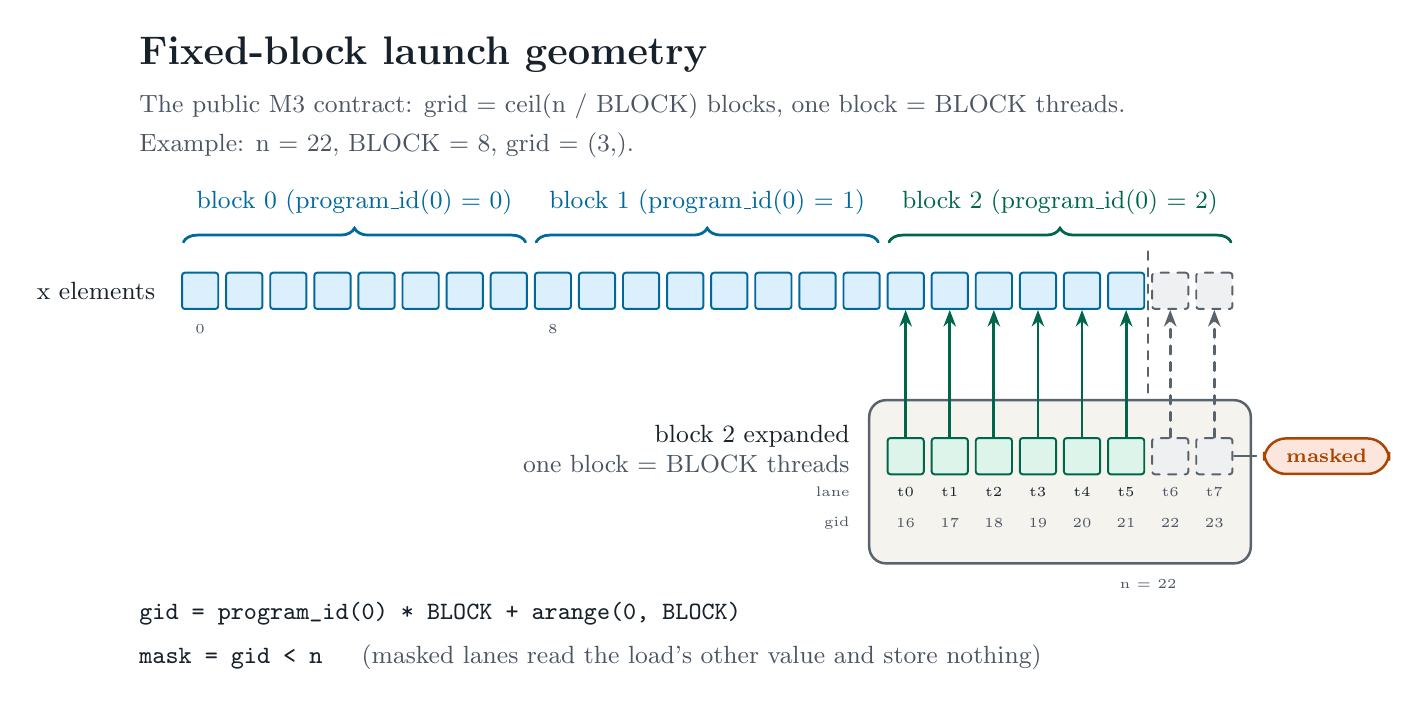
\begin{tikzpicture}[x=0.56cm, y=1cm]

% Header.
\node[swtitle] at (-1.6, 4.0) {Fixed-block launch geometry};
\node[swsubtitle] at (-1.6, 3.35)
  {The public M3 contract: grid = ceil(n / BLOCK) blocks, one block =
   BLOCK threads.};
\node[swsubtitle] at (-1.6, 2.85)
  {Example: n = 22, BLOCK = 8, grid = (3,).};

% Block braces above the element row.
\foreach \b/\lo/\hi in {0/0/7, 1/8/15} {
  \draw[decorate, decoration={brace, amplitude=5pt}, swblue,
        line width=1pt] (\lo - 0.38, 1.62) -- (\hi + 0.38, 1.62);
  \node[font=\small, text=swblue] at ({(\lo + \hi) / 2}, 2.12)
    {block \b\ (program\_id(0) = \b)};
}
\draw[decorate, decoration={brace, amplitude=5pt}, swgreen,
      line width=1pt] (15.62, 1.62) -- (23.38, 1.62);
\node[font=\small, text=swgreen] at (19.5, 2.12)
  {block 2 (program\_id(0) = 2)};

% Input elements 0..21 plus the two ghost slots the tail block covers.
\node[anchor=east, font=\small, text=swink] at (-0.8, 1.0)
  {x elements};
\foreach \i in {0,...,21} {
  \node[swcell, fill=swbluefill, draw=swblue] (v\i) at (\i, 1.0) {};
}
\foreach \i in {22,23} {
  \node[swcell, fill=swgrayfill, draw=swline, dashed] (v\i)
    at (\i, 1.0) {};
}
\foreach \i in {0, 8} {
  \node[font=\tiny, text=swmuted] at (\i, 0.52) {\i};
}

% The n boundary separates live elements from masked tail coverage.
\draw[swline, dashed, line width=0.8pt] (21.5, 1.5) -- (21.5, -2.5);
\node[font=\tiny, text=swmuted] at (21.5, -2.72) {n = 22};

% Expanded tail block: one lane per thread, directly under its element.
\node[swbox, fit={(15.55, -2.25) (23.45, -0.6)}, inner sep=6pt] {};
\foreach \t in {0,...,5} {
  \pgfmathtruncatemacro{\gid}{16 + \t}
  \node[swcell, fill=swgreenfill, draw=swgreen] (l\gid)
    at (\gid, -1.1) {};
  \node[font=\tiny, text=swink] at (\gid, -1.55) {t\t};
  \node[font=\tiny, text=swmuted] at (\gid, -1.95) {\gid};
  \draw[swarrow, draw=swgreen] (l\gid.north) -- (v\gid.south);
}
\foreach \t in {6,7} {
  \pgfmathtruncatemacro{\gid}{16 + \t}
  \node[swcell, fill=swgrayfill, draw=swline, dashed] (l\gid)
    at (\gid, -1.1) {};
  \node[font=\tiny, text=swmuted] at (\gid, -1.55) {t\t};
  \node[font=\tiny, text=swmuted] at (\gid, -1.95) {\gid};
  \draw[swarrow, dashed] (l\gid.north) -- (v\gid.south);
}
\node[swtag, draw=sworange, fill=sworangefill, text=sworange,
      anchor=west] at (24.1, -1.1) {masked};
\draw[swline, line width=0.8pt] (23.95, -1.1) -- (23.45, -1.1);

% Row labels for the expanded block.
\node[anchor=east, font=\small, text=swink] at (14.95, -0.85)
  {block 2 expanded};
\node[anchor=east, font=\small, text=swmuted] at (14.95, -1.2)
  {one block = BLOCK threads};
\node[anchor=east, font=\tiny, text=swmuted] at (14.95, -1.55) {lane};
\node[anchor=east, font=\tiny, text=swmuted] at (14.95, -1.95) {gid};

% The index and mask formulas the lanes implement.
\node[anchor=west, swcode] at (-1.6, -3.1)
  {\detokenize{gid = program_id(0) * BLOCK + arange(0, BLOCK)}};
\node[anchor=west, swcode] at (-1.6, -3.65)
  {\detokenize{mask = gid < n}~~~{\normalfont\small\color{swmuted}
   (masked lanes read the load's other value and store nothing)}};

\end{tikzpicture}
\end{document}
